\documentclass{article}

\usepackage{tikz}

\begin{document}

{
\centering
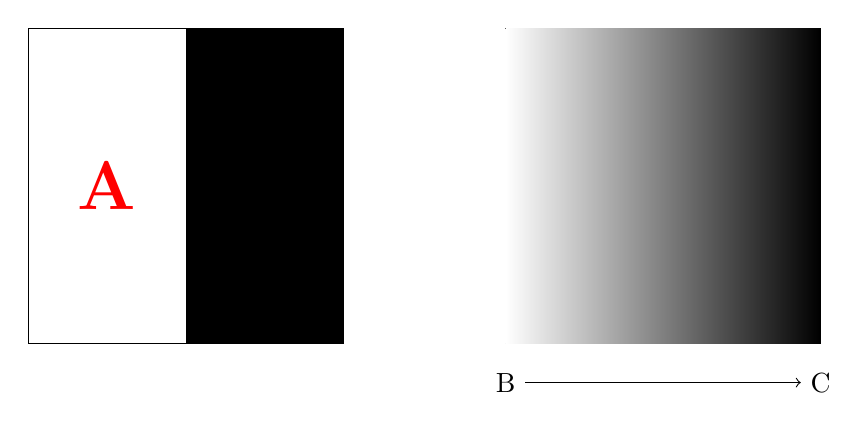
\begin{tikzpicture}
%Nodes
\draw (0,0) -- (4,0) -- (4,4) -- (0,4) -- (0,0);
\fill[black] (2,0) rectangle (4,4);
\node[red,font=\bfseries\Huge] at (1,2) {A};

\begin{scope}[xshift=.5\textwidth]
%Nodes
\draw (0,0) -- (4,0) -- (4,4) -- (0,4) -- (0,0);
\shade[left color=white,right color=black] (0,0) rectangle (4,4);
\node (B) at (0,-0.5) {B};
\node (C) at (4,-0.5) {C};
\draw[->] (B) -- (C) ;
\end{scope}
\end{tikzpicture}
}

\end{document}